\documentclass[11pt]{article}
\usepackage{amsmath}
\usepackage{mathbbol}
\usepackage{graphicx}
\graphicspath{{./}}

\title{INFORME DE LA PRÁCTICA PROFESIONAL 
FACULTAD DE MATEMÁTICA Y COMPUTACIÓN}
\author{
    \bf {Autor: Adrian Hernández Santos}\\
    \bf {Grupo: 211}\\
    \bf {Carrera: Ciencias de la Computación}\\
    \bf {Curso: 2022}\\
    \bf {Tutor: Damián Valdéz Santiago}\\
    \bf {Departamento de Matemática Numérica - MATCOM - UH}
}
\date{}

\normalsize
\begin{document}
\maketitle

\vfill
{
    \centering
    {
        \Large{\bf {Formulación de filtros de señales para identificar locutores auténticos e inauténticos}}
    }
}

\paragraph*{Resumen:} En este artículo se describe el proceso de formulación de filtros de señales para caracterizar 
los locutores auténticos e inauténticos que pudieran intervenir en la misma, utilizando transformadas wavelet y 
sistemas de ecuaciones simbolicas y no lineales.

\clearpage

\section*{Introducción}
El proceso de análisis de datos, específicamente de señales de diversa índole es necesario en casi todos los aspectos 
de la ciencia y la técnica. Dado a la utilización de equipos de cómputo en la gran mayoría de los procesos de la sociedad 
se hace inminente un método eficaz y preciso para transformar esos datos en conocimiento que aporte información que se pueda 
procesar. Con el auge de la Inteligencia Artificial y el Aprendizaje de Máquina, es muy frecuente su uso, pero dichos procesos requieren una cantidad enorme 
de datos iniciales para poder garantizar una respuesta acertada, algo que no es posible en algunos contextos. Por esta razón 
se ha optado por desarrollar un enfoque basado en modelos de optimización para obtener una solición de una calidad bastante similar 
pero reduciendo enormemente la cantidad de datos iniciales para modelar dicho problema. Llevando esta problemática especificamente 
a la detección de locutores en señales de audio, se propone una solucion utilizando un modelo basado en caracterización de 
dichas señales mediante filtros, dependientes de coeficientes de conocimientos únicos para un determinado conjunto de datos.

\clearpage

\section*{Descripción de la Institución}
\paragraph*{Departamento de Matemática Numérica, Facultad de Matemática y Computación, Universidad de la Habana:}
Grupo de investigación con soluciones a problemáticas utilizando Matemática Aplicada: procesos de optimización, ecuaciones diferenciales, métodos númericos, entre otros.


\clearpage

\section*{Descripción de las Actividades}
\paragraph*{Investigación:}
Durante esta fase, el objetivo fue la familiarización con el problema en cuestión: la necesidad de dado un conjunto de señales, determinar filtros que caractericen 
cualquier señal de un locutor en auténtico o inauténtico, con respecto a las señales de entrada. Utilizando la bibliografía relativa al problema se pudo dividir dicho problema en 
3 subproblemas mas pequeños, cuya unión da solución a la problemática inicial:

\section*{Subproblema 1:}
Dado un soporte de filtros \(N\), se deben hallar los filtros pasa-altas \(q[n]\) y pasa-bajas \(p[n]\). Dichos filtros quedarían en función 
de \(K = N - (\frac{N}{2} - 1)\) coeficientes de conocimiento. Este proceso no devuelve directamente los valores de \(q\) y \(p\) reales, sino que formarán un sistema de 
ecuaciones no lineal con dichos filtros en función de los coeficientes de conocimiento \(K\), los cuales se aplicarán a la descomposición de las señales. El algoritmo 
para formular dichos filtros \(q\) y \(p\) es el siguiente:

\noindent {\section*{\underline{INICIO}}}

\paragraph*{Paso 1:}
Los filtros \(q\) se esperan que tengan energia unitaria, por tanto, preservando la energia de la señal original se tiene que:
\begin{equation}
    \sum_{k=0}^{N - 1} q^2 = 1
\end{equation}

\paragraph*{Paso 2:}
\(\frac{N}{2}\) momentos nulos son aplicados, utilizados en la familia {\it wavelet} Symmlet:

\begin{equation}
    \sum_{k=0}^{N - 1} q_{k}(\frac{N}{2} + 1 + k)^b = 0
\end{equation}

Donde \(b = \{1, 2, ..., \frac{N}{2} - 1\}\)

\paragraph*{Paso 3:}
\(\frac{N}{2} - 1\) restricciones de clase son impuestas:

\begin{equation}
    \sum_{k=0, j=0}^{N - 1} q_{k}K_{j} = 0
\end{equation}

Donde \(K_{j}\) son los coeficientes de conocimiento.

\paragraph*{Paso 4:}
Las ecuaciones de los pasos 1, 2 y 3 son agrupadas formando un sistema de ecuaciones no lineal de \(N\) ecuaciones y \(N\) incógnitas que corresponden a 
los filtros pasa-altas \(q\). Dicho sistema de ecuaciones y por tanto sus soluciones no son numéricas, sino que quedan en función de \(K = N * (\frac{N}{2} - 1)\) 
incógnitas que serían los coeficientes de conocimiento.

\paragraph*{Paso 5:}
Una vez obtenidos los \(q[n]\) filtros en funcion de los \(K\) coeficientes de conocimiento podemos formular 
los \(N\) filtros pasa-bajas \(p[n]\) mediante la forma:

\begin{equation}
    p_{k} = (-1)^{k-1}q_{N - k - 1}
\end{equation}

\noindent {\section*{\underline{FIN}}}

\section*{Subproblema 2:}
Teniendo los filtros \(q\) y \(p\) en función de los \(K\) coeficientes de conocimiento, se hace necesario obtener dichos coeficientes. Para lo cual se tiene una entrada de \(M : M = N\) 
señales numéricas. Realizando el producto matricial \(As = r\), donde \(A[n \times n]\) representa una matriz de {\it Cuadratura de Filtros Espejados}, formulada a partir de 
\(q[n]\) y \(p[n]\); \(s[n]\) es una señal numérica de entrada, con las muestras del contenido a filtrar; y \(r[n]\) la señal transformada esperada. Dicho proceso es llamado {\it Algoritmo 
de Mallat}, el cual es un algoritmo de {\it Transformada Discreta Wavelet}. Consiste en una multiplicación de dicha matriz de cuadratura, por una señal de entrada, donde el resultado de concatenar 
los \(\frac{N}{2}\) indices pares de \(r[n]\) con los \(\frac{N}{2}\) indices impares corresponde al primer nivel de la {\it Transformada Discreta Wavelet} sobre \(s[n]\). Realizando este proceso \(\log_{2}{N}\) 
veces, hasta que la señal de entrada tenga solamente un único coeficiente, obtenemos la transformada de dicha señal, donde en cada iteración se reformula la matriz \(A\), atendiendo al tamaño de la entrada 
del nivel correspondiente de la transformada. Para la solución de este subproblema se propone el siguiente algoritmo:

\noindent {\section*{\underline{INICIO}}}

\paragraph*{Paso 1:}
Formulamos la matriz de cuadratura de filtros espejados \(A\) en función de \(p\), \(q\) y \(M\) de la siguiente forma:

\begin{equation}
    \begin{pmatrix}
        q_0 & q_1 & q_2 & q_3 & q_4 & ... & q_{M - 1} & 0 & ... & 0\\ 
        p_0 & p_1 & p_2 & p_3 & p_4 & ... & p_{M - 1} & 0 & ... & 0\\ 
        0 & 0 & q_0 & q_1 & q_2 & ... & 0 & q_{M - 1} & ... & 0\\ 
        0 & 0 & p_0 & p_1 & q_2 & ... & 0 & p_{M - 1} & ... & 0\\ 
        ... & ... & ... & ... & ... & ... & ... & ... & ... & ...\\
        ... & ... & ... & ... & ... & ... & ... & ... & ... & ...\\
        q_2 & q_3 & ... & ... & q_{M - 1} & 0 &... & 0 & q_0 & q_1\\
        p_2 & p_3 & ... & ... & p_{M - 1} & 0 &... & 0 & p_0 & p_1\\
    \end{pmatrix}
\end{equation}

\paragraph*{Paso 2:}
Usamos el {\it Algoritmo de Mallat} para hallar \(TDW_{s[M]}\) {\it (Transformada Discreta Wavelet para \(s[M]\))}, realizando el producto matricial:

\begin{equation}
    A \times s = r
\end{equation}

Proceso que se repite \(\log_{2}N\) veces, donde luego de cada vez que efectua el producto el primer nivel de la 
\(TDW_{s}\) quedaría como la concatenación de los índices pares e impares del resultado \(r\) de la forma: \(r = \{r_{0}, r_{2}, r_{4}, ..., r_{N - 2}, r_{1}, r_{3}, r_{5}, ..., r_{N - 1}\}\), ya que se espera 
que la entrada \(N\) siempre sea par.

\paragraph*{Paso 3:}
Luego, cada nivel subsecuente de la \(TDW_{s}\) sería el resultado de aplicar el {\bf Paso 2} a los \(\frac{N}{2}\) resultados del nivel anterior, hasta llegar al nivel \(\frac{\log_{2}M}{2}\), con el cual obtenemos la transformada de 
nivel medio de la señal original \(s\).

\noindent {\section*{\underline{FIN}}}

\section*{Subproblema 3:}
Luego de tener las señales transformadas de nivel medio, se hace necesario caracterizar dichas señales. Para dicha caracterización se pueden utilizar distintas funciones que permitan apreciar las propiedades físicas de las señales 
transformadas: para este trabajo hemos seleccionado {\it Skewness (Asimetría)} y {\it Kurtosis (Curtosis)}. Aplicando dicha caracterización de propiedades físicas a cada \(Z_{i}[.]\), que representan las sub bandas de frecuencia del proceso de descomposición 
con {\it Transformada Wavelet Discreta} de nivel medio, se puede formular un \(\lambda\) para cada fenomeno físico a caracterizar, que permite filtrar dichos resultados y crear una especie de punto de ruptura para formar nuestra caracterización en locutores auténticos e 
inauténticos. Tomando los \(Z_{i}[.]\) que corresponden a las transformadas de frecuencias mayores a 1 kHz, podemos calcular una media \(\mu_{AF}\) y la desviación estándar \(\sigma_{AF}\). El siguiente algoritmo permite formular el segundo 
sistema de ecuaciones no lineal que permite obtener el valor de los coeficientes de conocimiento \(K\):

\noindent {\section*{\underline{INICIO}}}
\paragraph*{Paso 1:}
Sea \(f = Skewness \) función que modela las propiedades asimétricas de una señal y \(Z_{i}[.]\) el i-ésimo elemento de la transformada de nivel medio de \(s\) de altas frecuencias:

\begin{equation}
    \mu_{AF} = \frac{\sum_{i=1}^{2^{\log_{2}(M - J)} - 1} f(Z_{i}[.])}{2^{\log{2}(M - J)} - 1}
\end{equation}

\begin{equation}
    \sigma_{AF} = \frac{\sum_{i=1}^{2^{\log_{2}(M - J) - 1}}(f(Z_{i}[.]) - \mu )^2}{2^{\log{2}(M - J)} - 1}
\end{equation}

\begin{equation}
    \lambda_{kur} = \mu_{AF} + 2 \times \sigma_{AF}
\end{equation}

\begin{equation}
    \lambda_{skw} = \mu_{AF} + \sigma_{AF}
\end{equation}

Donde \(M\) = tamaño de la transformada \(Z\) de nivel medio y \(J\) la cantidad de muestras de \(Z\) con frecuencias menores que 1 kHz.

\paragraph*{Paso 2:}
En función de esos \(\lambda\), se pueden agrupar las señales \(Z\) de tal forma que se puedan filtrar los auténticos de los inauténticos:

\begin{equation}
    \begin{cases}
        {\bf Aut\acute{e}nticos} & \text {\(f(Z_{0}[.]) <= \lambda\)}\\
        {\bf Inaut\acute{e}nticos} & \text{\(f(Z_{0}[.]) > \lambda\)}\\
    \end{cases}
\end{equation}

\paragraph*{Paso 3:}
Para formular el segundo sistema no lineal, cuya solución serán los coeficientes \(K\), se toman las señales de entrada que pasan por el proceso de descomposición usando los filtros \(q\), 
se formula una ecuación de caracterización de conocimiento, o sea, el número de señales de entrada implica el número de ecuaciones que componen el segundo sistema no lineal y su solución: 
los coeficientes \(K\).

\paragraph*{Paso 4:}
Una vez solucionado el sistema no lineal del {\bf Paso 4} y obtenidos los \(N \times (\frac{N}{2} - 1)\) coeficientes de conocimiento \(K\), se sustituyen esos valores numéricos en las ecuaciones simbólicas \(q\), o sea 
\(q(k_{0}, k_{1}, ..., k_{N \times (\frac{N}{2} - 1) -1})\), cuyo resultado produciría los \(N\) coeficientes numéricos \(q_{i}\) de los filtros basados en conocimiento.

\noindent {\section*{\underline{FIN}}}

\clearpage

\section*{Conclusiones}
Durante el tiempo de la práctica laboral, se realizaron investigaciones y experimentos en el ámbito del procesamiento de señales, cuestiones que no se tratan en el plan de estudio básico de la carrera Ciencias de la Computación, 
pero que contienen un alto contenido teórico/práctico que es de amplio uso e importancia en muchos sectores de la ciencia y la técnica, que es a fin de cuentas, el objetivo principal en la formación de un estudiante. A pesar de que, 
por cuestiones de tiempo, solamente se pudo abarcar una solución del problema principal hasta el {\bf Subproblema 2}, el resto queda para una posterior etapa de prácticas laborales, donde se ampliará aún más sobre el tema. Se intentará 
mejorar las soluciones iniciales e incluso lograr una solución general para el mismo, utilizando un enfoque similar al del problema en cuestión. A pesar de esto, la investigación realizada ha aportado conocimientos extra de asignaturas como 
{\it Álgebra, Análisis Matemático, Matemática Numérica y Programación}, así como un acercamiento a problemáticas de la vida real y como se hayan soluciones prácticas a estas. 

\clearpage

\section*{Anexos}

\paragraph*{Transformada Symmlet:}
Familia {\it wavelet} con amplio uso en el tratamiento de señales de voz, debido a que su forma refleja bastante bien las características principales de la voz.

\paragraph*{Transformada Discreta Wavelet:}
Una {\it wavelet} o forma de onda, es una señal que tiene una duración limitada y un valor promedio de 0. La principal diferencia con la transformada de Fourier, para el análisis de señales son sus propiedades de asimetría e irregularidad, las cuales describen 
mucho mejor el comportamiento real de una señal, ya sea analógica o digital. Al seleccionar una {\it wavelet} de las distintas familias existentes, por su similitud con el tipo de señal que queremos analizar, se le pueden realizar cambios, puesto que esta puede trasladarse 
o escalar (comprimirse o expandirse) a lo largo de nuestra señal. Si definimos nuestra wavelet como \(\psi_{a, b}(t)\), siendo \(a\) y \(b\) los parámetros de escalamiento y desplazamiento respectivamente se tiene:

\begin{equation*}
    \psi_{a,b}(t) = \frac{1}{\sqrt{a}}\psi(\frac{t - b}{a})
\end{equation*}

Teniendo esto podemos definir la {\it Transformada Continua Wavelet} como el producto de una señal continua y su {\it wavelet} asociada en su versión desplazada y escalada de la forma:

\begin{equation*}
    TCW(a, b) = \frac{1}{\sqrt{a}}\int_{-\infty}^{\infty}x(t)\psi(\frac{t - b}{a})dt
\end{equation*}

donde \(x(t)\) es la señal continua.\\
La TDW se obtiene al discretizar los parámetros de desplazamiento y escalamiento dentro de la TCW. Generalmente los valores que se utilizan son:

\begin{equation*}
    \begin{cases}
        a=2^{-j}\\
        b=k2^{-j}
    \end{cases}
\end{equation*}

donde \(a\) es el escalamiento, \(b\) el desplazamiento y \(j, k\) valores enteros. Dado esto se tiene que la nueva {\it wavelet} queda de la forma:

\begin{equation*}
    \psi_{j, k}(t)= w^{\frac{j}{2}}\psi(2^{j}t - k); j, k \in \mathbb{Z}
\end{equation*}

Por lo que con lo anterior podemos definir la TDW como:

\begin{equation*}
    TDW_{j, k} = 2^{\frac{j}{2}}\int_{-\infty}^{\infty}x(t)\psi(2^{j}t-k)dt
\end{equation*}

con \(x(t)\) una señal discreta. 

\paragraph*{Filtro de convolución (pasa-bajas o pasa-altas):}
Expresión cuya función principal es atenuar las señales de bajas(altas) frecuencias, para concentrarse en las de altas(bajas) frecuencias. El proceso de convolución esta dado por la transformación de 2 señales digitales en una tercera, basándose en ciertas 
características y con un objetivo específico, dependiendo de la transformada que se utilice en el proceso.

\paragraph*{Cuadratura de Filtros Espejados:}
Matriz de convolución asociada a los filtros pasa-bajas y pasa-altas, en la que cada par de filas contiene a dichos filtros, con un desfase de 2 columnas con respecto al par de filas anterior y rellenando todos los demás espacios vacíos con 0. Esta matriz de convolución, 
se utiliza pa hacer {\it downsampling} a la señal de entrada usando el método de {\it Transformada Discreta Wavelet} descrito en el algoritmo de Mallat, con modificaciones para adaptarlo al contexto de señales de sonido.

\paragraph*{Algoritmo de Mallat:}
Stephane G. Mallat, en su artículo: "{\it A Theory for Multiresolution Signal Decomposition: The Wavelet Representation}", plantea una forma de descomponer señales de una y dos dimensiones relacionadas a imágenes, utilizando {\it Transformadas Wavelet}, para facilitar el análisis 
de distintas propiedades de dichas imágenes. Este proceso se basa en una formulación, utilizando las bases ortonormales respectivas a una {\it wavelet}, para formular un sistema piramidal, en el cual utilizando un banco de filtros \(H y G\) pasa-bajas y pasa-altas, se puede 
hacer {\it downsampling} de la señal original para su posterior clasificación, disminuyendo su resolución, pero sabiendo en todo momento el cambio de sus propiedades con respecto a una resolución anterior. Este proceso es válido incluso en sentido inverso, realizando un {\it upsampling}, para 
revertir el proceso, e incluso recrear dichas imágenes (señales), a partir de otras descomposiciones. En este informe y algunos de los citados, se utiliza una adaptación de ese algoritmo, para realizar la descomposición de una señal de entrada, para su posterior clasificación utilizando 
Asimetría ({\it Skewness}) y Curtosis ({\it Kurtosis}), para obtener un parámetro de clasificación basado en conocimiento y encontrar la solución al problema inicial.

\paragraph*{Skewness:}
Propiedad probabilística que clasifica una distribución en cuanto a su asimetría con respecto a su media. Su forma es muy similar a la distribución de Poisson.

\paragraph*{Kurtosis:}
Propiedad probabilística que clasifica una distribución con respecto a que tan concentrada esta con respecto a su media. En un valor promedio se puede apreciar una similitud con la distribución Normal o Gaussiana.

\pagebreak

\begin{figure*}
    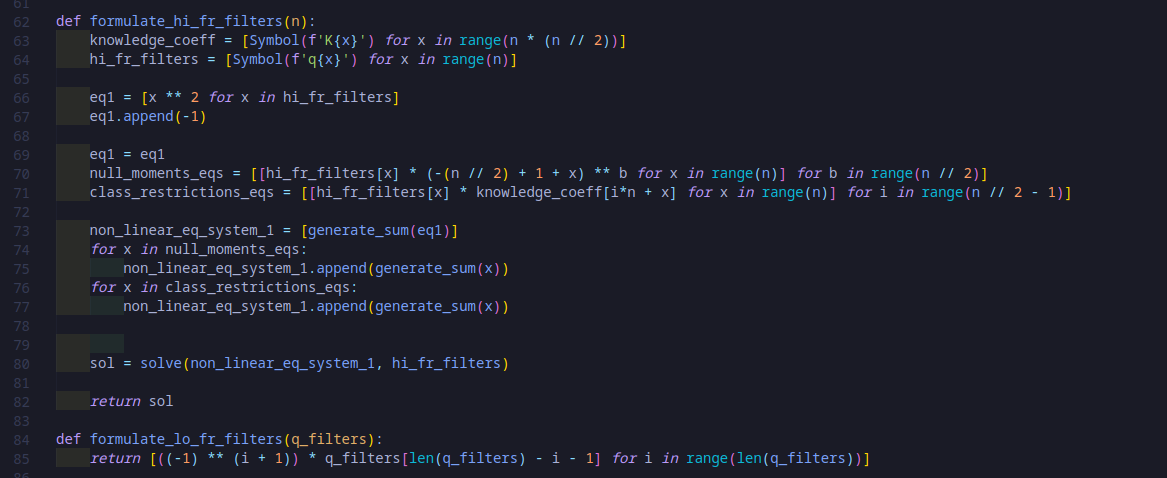
\includegraphics[width=\textwidth]{filters}
    \caption{\it Código utilizado en la formulación de los filtros simbólicos basados en conocimiento.}
\end{figure*}

\begin{figure*}
    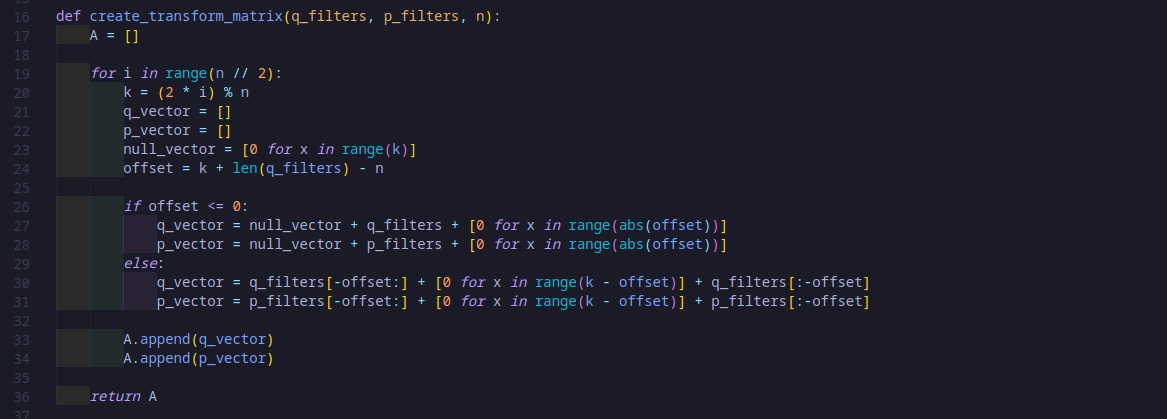
\includegraphics[width=\textwidth]{filter_bank}
    \caption{\it Código utilizado para crear la matriz de Filtros Espejados para el proceso de downsampling.}
\end{figure*}

\begin{figure*}
    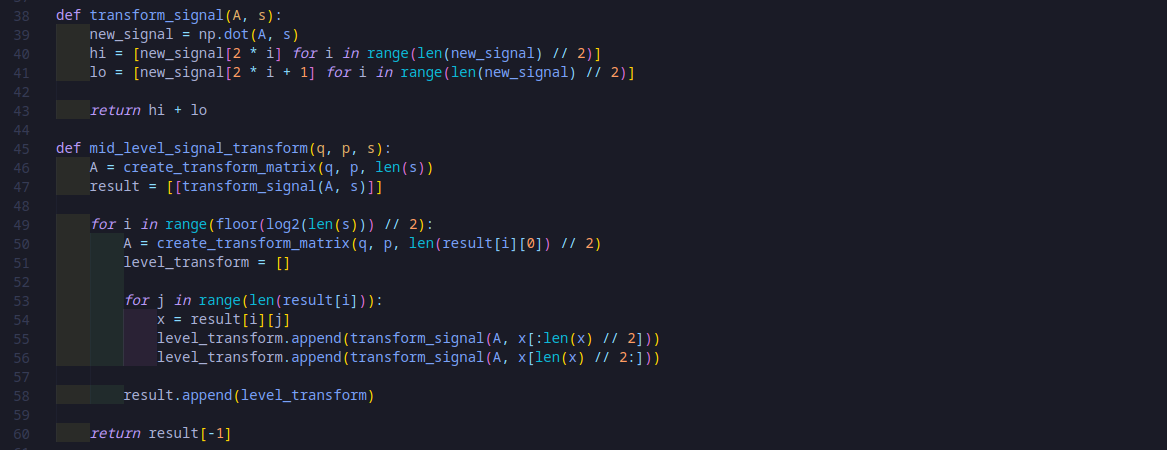
\includegraphics[width=\textwidth]{transform}
    \caption{\it  Código utilizado para realizar la transformación de nivel medio a la señal de entrada, utilizando el algoritmo planteado en el {\bf Subproblema 2}}
\end{figure*}


\clearpage

\section*{Bibliografía}
\begin{enumerate}
    \item Almeida, Guido (2022): {\it Elaboração de filtros Wavelet baseada em
    conhecimento para distinção entre locutores
    autênticos e inautênticos}, São José do Rio Preto
    \item Almeida, Guido (2021): {\it Knowledge-Based Wavelet Filters Prominently
    Detect Spoofed Speech}, São José do Rio Preto
    \item S.G Mallat, (1987): {\it A Theory for Multiresolution Signal Decomposition: The Wavelet Representation}, IEEE Transactions on Pattern Analysis and Machine Intelligence
    \item Westfall, Peter H. (2015): {\it Kurtosis as Peakedness, 1905 – 2014. R.I.P.}, The American Statistician
    \item Weisstein, Eric W.: {\it Skewness}, Wolfram Research
    \item Grupo de Investigación en Sistemas Inteligentes, Facultad de Estudios Superiores Cautitlán (2018): {\it Transformada wavelet}, Universidad Nacional Autónoma de México
\end{enumerate}

\end{document}